\documentclass{article}
\usepackage{latexsym}
\usepackage{amssymb,amsmath}
\usepackage{custom2}
\usepackage{graphicx} % for figures
\usepackage{epstopdf} % so can use EPS or PDF figures
\usepackage{caption}
\usepackage{subcaption}
\usepackage{url}
\usepackage{amssymb,amsfonts}
\usepackage[all,arc]{xy}
\usepackage{enumerate}
\usepackage{mathrsfs}
\usepackage{booktabs}
\usepackage[pdftex]{hyperref}
\usepackage{lscape}
\usepackage{xcolor}
\usepackage{natbib}

\captionsetup{justification=RaggedRight, singlelinecheck=false}
\newcommand{\ra}[1]{\renewcommand{\arraystretch}{#1}}
\newcommand{\argmax}{\text{argmax}}
\newcommand{\Tr}{\text{Tr}}
%\newtheorem{claim}{Claim}
\newtheorem{ass}{Assumption}

\addtolength{\evensidemargin}{-.5in}
\addtolength{\oddsidemargin}{-.5in}
\addtolength{\textwidth}{1.4in}
\addtolength{\textheight}{1.4in}
\addtolength{\topmargin}{-.5in}

\pagestyle{empty}

\begin{document}
\begin{center}
\Large

\end{center}


\vspace{0pt}

\begin{center}
{\bf \LARGE{Stochastic Learning Dynamics with Two Applications}}
\end{center}

\tableofcontents

\section{Abstract}
Learning usually occurs in noisy environments.  In order to make a decision, one must accumulate the  evidence for different alternatives and choose one only once the uncertainty about the choice is sufficiently reduced.  There are two equivalent mathematical formulations of the optimal decision making algorithm: a sequential probability ratio test in which the likelihoods of two hypotheses are evaluated as more data points are collected and a drift-diffusion stochastic differential equation in which the belief about two hypotheses does a random walk until a threshold is reached.  In the random walk formulation, the threshold dictating when a decision has been made affects both the accuracy of the decision and the expected time until a decision is reached.  If the utility of a decision depends on accuracy and decision time, the threshold can be optimized accordingly.  There are two biological systems in which the variables used to make a decision can be described by a random walk: the firing rates of neural populations in the brain of an individual making a decision about a visual stimulus and the beliefs of monkeys about their relative dominance based on the fights they have engaged in.  The stochastic differential equations used to model these quite different systems are nearly identical, which suggests that there are universal principles underlying learning through noisy dynamical systems in biology.  However, there are (at least) three significant differences between the two models.  First, in the social system, there is a strategic component to the system since the optimal threshold of one animal depends on the threshold of the other animal, whereas in the neural system both neural populations are part of the cognitive system of the same individual trying to optimize its decision making.  Relatedly, the output of the decision has additional strategic consequences in the social system.  Second, whereas in the neural system, the differential equations are often reduced to a one-dimensional model, the social system is inherently two-dimensional.  Finally, in the social system, a monkey is not only trying to make a decision about his dominance with respect to one other monkey, but he is additionally trying to make decisions about many other partners at once, whereas in the neural case there is only one decision to be made at a time.  As a consequence of these differences... In comparing the output of the model of the social system to data, we found that ...

\section{Introduction}

\subsection{Neural }
Stochastic differential equations have been used to model, explain, and predict learning and decision making in both monkeys and humans \citep{Eckhoff:2008uq, Brown:2005fk,Feng:2009kl,Bogacz:2006uq}.  Typically, an experimental subject is presented with a visual stimulus that consists of dots, some percentage of which are moving coherently either left or right and the rest of which are moving randomly.  The subject is then asked to decide in which direction the dots were moving.  If there are two neural populations, each of which fire in response to a particular direction of motion, the firing rates of the two populations will tend to increase or decrease, depending on the strength and direction of the stimulus.  Eventually, either the experimenter forces a decision to be made, in which case whichever population has a higher firing rate determines which decision is made, or the firing rate of one population becomes high enough that the subject decides for that direction.  To summarize, there are two decision variables--- the firing rates of two neural populations responding to left and right motion--- that perform a biased random walk until enough evidence has been accumulated to make a decision one way or the other.


\subsection{Social }
In groups of pigtailed macaques, different animals have different fighting abilities, and when a pair of animals engages in a fight, one animal may be more likely on average to ``win" the fight.  Over time, as one animal learns that it is likely to lose fights, it will decide to emit a formal subordination signal, communicating its agreeing to the subordinate role in their relationship \citep{Flack:2007kx, Flack:2006fk,Flack:2004oq, Waal:1985fk,Caldecott:1986uk}.  The outcome of a fight is affected by each animal's allies, the presence of those allies, motivation levels,  external environmental variables, and other factors.  Additionally, the number of fights that occur in any period of time depends on similarly stochastic factors.  Because of this stochasticity, the number of fights won and lost in any period of time is a random variable.  Each animal's opinion about its relative dominance, therefore, will perform a biased random walk until one animal's opinion of itself is low enough to agree to being subordinate.

Similar models have previously been applied to animal conflicts, although in that case the animals had perfect memory of their past interactions \citep{Froment:2010fk}

\subsection{Extent and Limits of Analogy }

In Table \ref{analogy}, we list the inputs, decision variables, and outputs of the two systems.  

\section{Derivation of Model \label{derivation}}
Stochastic differential equations have been phenomenologically applied to learning systems, with some success \citep{Eckhoff:2008uq, Brown:2005fk,Feng:2009kl,Bogacz:2006uq}.  However, with two assumptions about the timescales on which probabilistic events occur, a simple mechanistic description of the accumulation of information about random events can be turned into a stochastic differential equation \cite{Gillespie:2000fk}.  

\begin{equation}
\begin{array}{ll}
dX_1&=\bigg(-\ell X_1(t)+b(2d-1)\bigg)dt+b\sqrt{d}dW_{1}t-b\sqrt{(1-d)}dW_{2}t
\\dX_2&=\bigg(-\ell X_1(t)+b(1-2d)\bigg)dt-b\sqrt{d}dW_{1}t+b\sqrt{(1-d)}dW_{2}t,
\end{array}
\end{equation}

In Table \ref{models}, we compare 

A drift diffusion model is equivalent to a sequential probability ratio test, a learning algorithm that is optimal with respect to its accuracy and the time required to make a decision \cite{Moehlis:2004fk,Bogacz:2006uq}.  

The outcome of the decision process is not deterministic. Because of the noise in this system, the utility of a decision depends on the probability of reaching the correct decision and the expected time it takes to reach a decision.  These quantities satisfy partial differential equations with respect to the starting values of the decision variables. In Appendix \ref{pdes_deriv}, we derive these partial differential equations.  While an analytical solution is known in the one-dimensional case, the two-dimensional case is analytically intractable.  We therefore numerically solve the PDEs in the two-dimensional case.

\section{Results}

\subsection{Two-Dimensional Decision Making }
In the neural system, the two stochastic equations describing the activity of the two neural populations integrating environmental evidence are often reduced to a one-dimensional equation describing the difference in the activity levels to make the system easier to analyze \cite{Brown:2005fk,Bogacz:2006uq,Feng:2009kl}.  However, in the social system we are considering, we cannot make any assumptions about the existence of a third party evaluating the difference in the opinions of the two animals.  A ``decision," i.e. the emission of a signal from one of the two animals, is only reached when one of the two animals' opinions goes below a certain threshold.  The social system is therefore inherently two-dimensional, whereas the neural system may be adequately described by one dimension. 

We can compare the decision making process in the full two-dimensional system and in a reduced one-dimensional system to see whether decisions are made more accurately or quickly in one or the other. We find that the two-dimensional decision is less accurate than the one-dimensional decision.  That is, for a given expected time to reach a decision, the two-dimensional decision will reach the correct decision with a lower probability (Figure \ref{1dv2d}).  The difference in probability is very low when memory is perfect (i.e. $\ell=0$).  However, at higher leak rates the difference becomes more pronounced.  Further, when the strength of the input ($d$) is lower, the difference becomes greater.  Thus, as the decision becomes harder because either memory decreases or the true state of the world becomes harder to detect, the advantage of the one-dimensional system increases.

\subsection{Strategic Decision Making }
Differences in the threshold between animals could just be explained by individual variation.  However, there may be a strategic aspect to this variation in the social system.  In the neural system, an individual wants to make both a decision that is both quick and accurate.  This is also true in the social system.  However, it may also be the case that a monkey wants to avoid emitting a subordination signal and wants to receive a signal, regardless of whether or not this is the ``correct" outcome, i.e. whether or not he is actually more likely to win a fight.  The criterion used to optimize the threshold, therefore, may be quite different in the two systems.  Additionally, the speed and outcome of the decision process depend on both animals' thresholds.  Since an animal's best behavior depends on the behavior of the other animal, optimizing the threshold is strategic in the social system but not in the neural system.  

\subsection{Social Decision Making }
A monkey can try to decide whether it is more or less likely to win a fight than another monkey using information from the fights the pair has previously engaged in.  Further, he can try to make such a decision about every other member of its social group.  Since he is trying to use the same algorithm to learn about every other animal, he is constrained to have only one decision threshold for each of these decision processes.  The optimal decision threshold in this social context depends on the distribution of fighting abilities in the group and the decision thresholds of the other animals. 

\subsection{Comparison to Social Data }
Empirically, those pairs of monkeys that take the longest to establish a signaling dynamics are those with the most similar fighting abilities...

\section{Discussion}


\section{Appendix}

\subsection{Derivation of PDEs for waiting time and accuracy \label{pdes_deriv}}

\begin{figure}
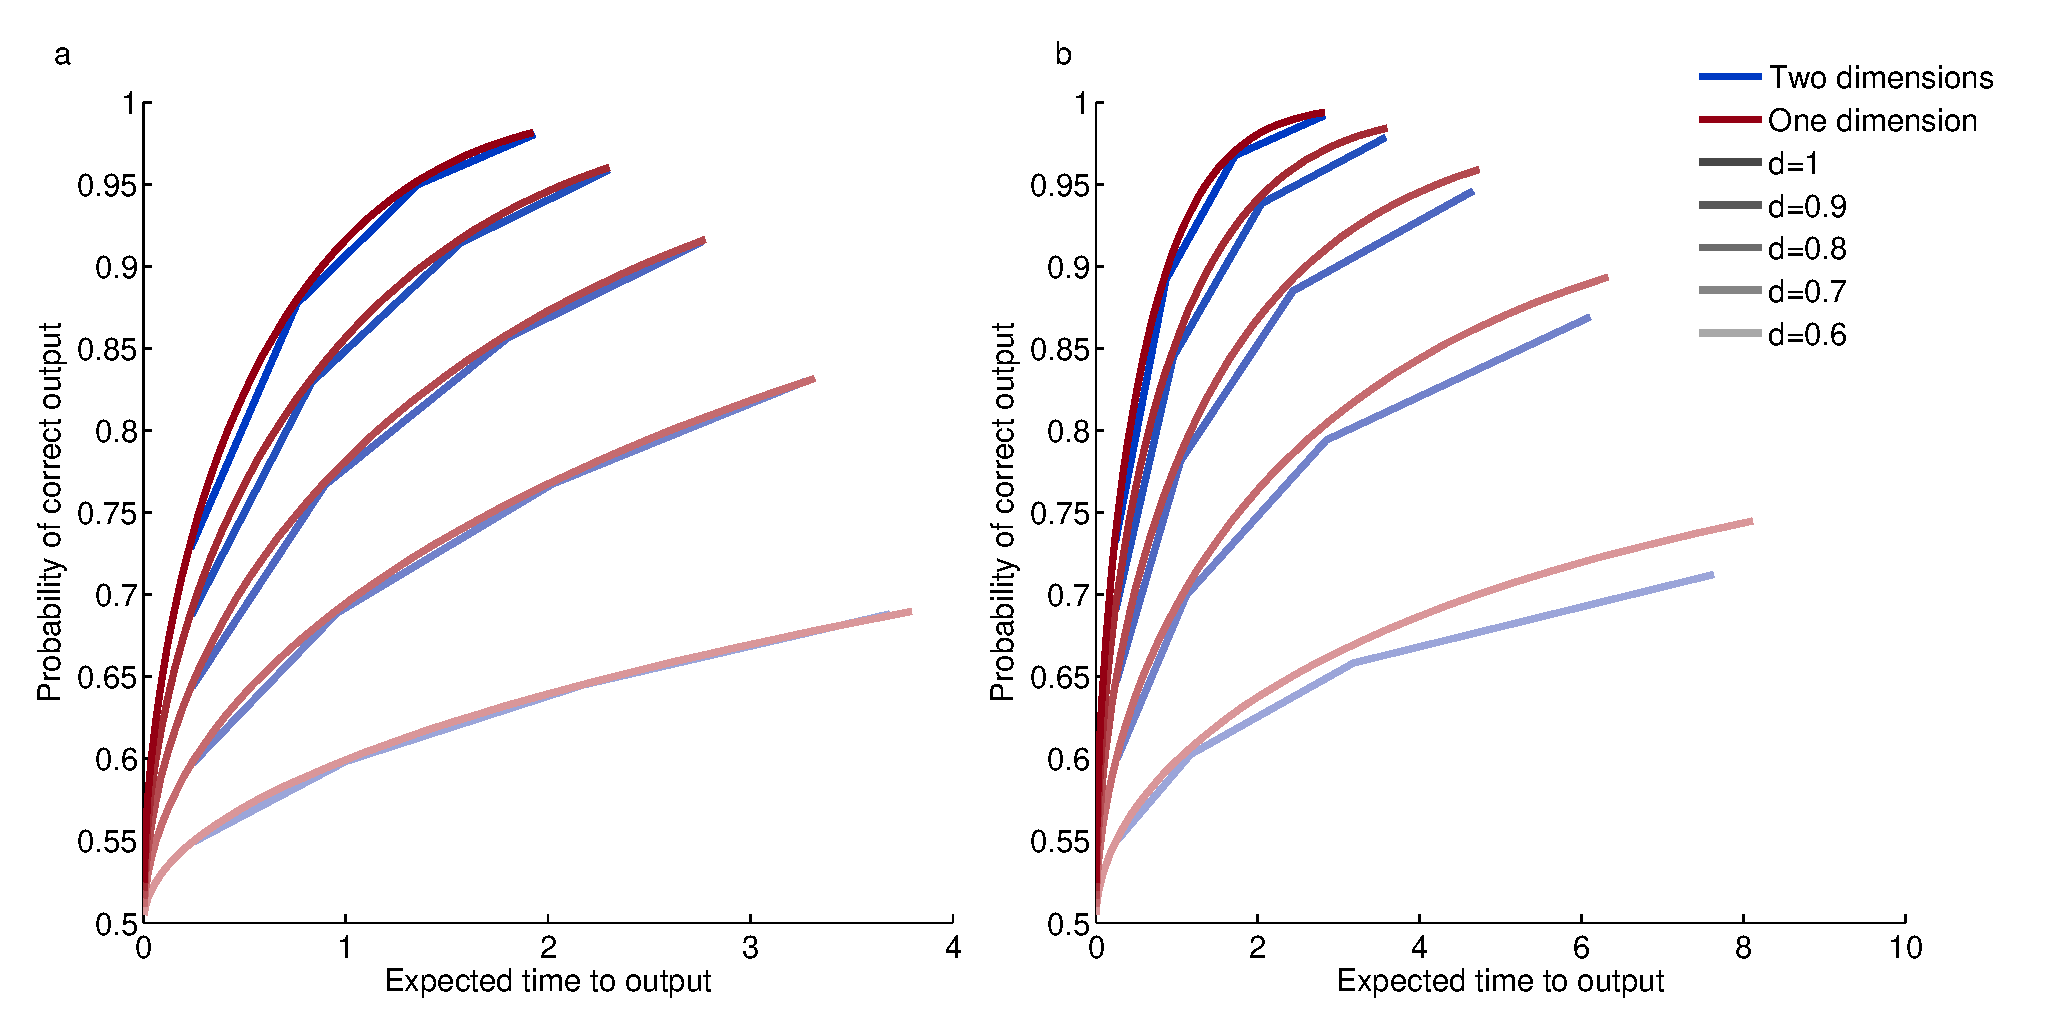
\includegraphics[width=\textwidth]{1d_v_2d_symmetric.pdf}
\caption{\label{1dv2d} A two-dimensional decision process, in which the decision is made when either of the variables reaches a threshold, is less accurate than a one-dimensional decision process, in which the decision is made when the difference between the variables reaches a threshold.  In each panel, the expected time to reach a decision is on the x-axis and the probability of reaching the correct decision in that amount of time is on the y-axis.  Red curves represent a one-dimensional decision and red curves represent a two-dimensional decision.  Stronger values of the input are represented in higher darker curves.  In the left panel, there is no leak.  In the right panel, leak rate is set to $\ell=.5$.  Other parameters are set as follows:}
\end{figure}

\begin{figure}
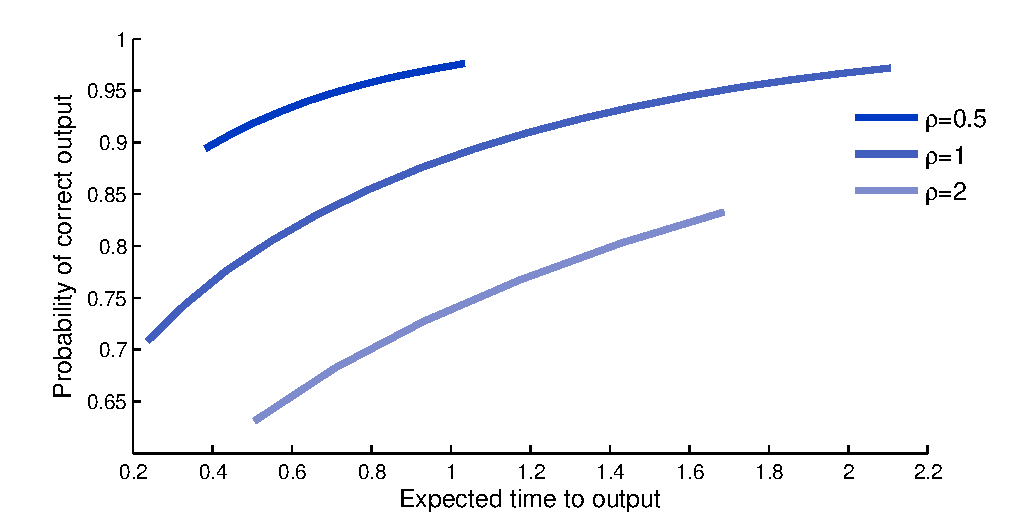
\includegraphics[width=\textwidth]{2d_flexible_thresholds.pdf}
\caption{\label{2dthresh} When the two thresholds in the two-dimensional case are allowed to vary freely, the decision process can be arbitrarily accurate in a given amount of time, depending on how much lower the weaker animal's threshold is than the stronger animal's threshold.  The expected time to reach a decision is on the x-axis and the probability of reaching the correct decision in that amount of time is on the y-axis.}
\end{figure}

\begin{table}
\centering
\caption{\label{analogy}{\bf  Analogy between neural and social systems.} }
\ra{1.3}
\begin{tabular}{@{}rllll@{}}
&Neural &   Social \\
\cmidrule{2-2} \cmidrule{3-3} 
input & dots moving left or right & fights won or lost
\\strength of input & coherence of dots & probability of stronger animal winning
\\decision variables &  firing rates of neural populations & opinions about relative dominance
\\ dist. of states of the world & left / right equally likely & distribution of fighting abilities
\\ decision & subject indicates left or right & one animal emits a subordination signal
\\ correct decision & subject chooses correct direction & weaker animal signals
\end{tabular}
\end{table}

\begin{table}\centering
\caption{\label{models}{\bf  Comparison of models applied to neural and social systems.} }
\ra{1.3}
\begin{tabular}{@{}rllll@{}}
& \multicolumn{2}{c}{Neural} & \phantom{abc}& Social \\
\cmidrule{2-3} \cmidrule{5-5} 
%model  & DDM or OU & race && race with leak
%\\
dimensionality & $1$ & $2$ && $2$
\\decision & difference hits a threshold & one var. hits a threshold && \fcolorbox{red}{white}{one var. hits a threshold}
\\ optimality criterion &  reward from being ``right" &&& reward from being ``right"
\\ & reward rate &&& reward rate
\\ & Bayes risk &&& Bayes risk
\\ & &&& \fcolorbox{red}{white}{reward from  receiving signal}
\\optimization depends on & input strength &&& input strength
\\ & noise &&& noise
\\ & leak rate &&& leak rate
\\ & &&& \fcolorbox{red}{white}{other animal's threshold}
\\threshold  algorithm & error correction
\\  & hill climbing
\end{tabular}
\end{table}

\nocite{*}
\bibliographystyle{plain}
\bibliography{signaling_model}

\end{document}


